%% FEUP THESIS STYLE for LaTeX2e
%% how to use feupteses (English version)
%% FEUP, JCL & JCF, October 2024
%%
%% Read the documentation inline and at the included `README` file
%%
%% PLEASE send improvements to jcf at fe.up.pt and to jlopes at fe.up.pt
%%

\documentclass[11pt,a4paper]{report}

%% For two-sided printing (for dead-tree output) comment previous line
%% and uncomment the next line
%\documentclass[11pt,a4paper,twoside,openright]{report}

%% Source text uses in UTF-8 encoding
\usepackage[utf8]{inputenc}

%% MEEC options
\usepackage[meec]{feupteses}              % working version
%\usepackage[meec,juri]{feupteses}        % juri version
%\usepackage[meec,final]{feupteses}       % final PDF version

%% Additional options for feupteses.sty:
%% - portugues: titles, etc in portuguese
%% - onpaper: links are not shown (for paper versions)
%% - backrefs: include back references from bibliography to citation place
%% - iso: format references according to ISO 690 standard

%% TIP: use folder ``figures'' to keep all your figures
%% Path to the figures directory
\graphicspath{{figures/}}

%% Change to the appropriate bibliography file
\addbibresource{bibliography.bib}

%%========================================
%% Start of document
%%========================================
\begin{document}

%%----------------------------------------
%% Information about the work
%%----------------------------------------
\title{$<$Dissertation Title$>$}
\author{$<$Author's Full Name$>$}

%% Uncomment next line for date of submission
%\thesisdate{July 31, 2008}

%% Comment next line copyright text if not used
\copyrightnotice{Name of the Author, 2008}

\supervisor{Supervisor}{Prof.\ $<$Name of the Supervisor$>$}

%% Uncomment next line if necessary
%\supervisor{Second Supervisor}{Prof.\ $<$Name of the Supervisor$>$}

%% Uncomment committee stuff in the final version if used
%\committeetext{Approved in oral examination by the committee:}
%\committeemember{President}{Prof.\ $<$Name of the Professor$>$}
%\committeemember{Referee}{Prof.\ $<$Name of the Professor$>$}
%\committeemember{Referee}{Prof.\ $<$Name of the Professor$>$}

%% uncomment next line to draw line for handwritten signature (if necessary)
%\signature

%% Specify cover logo (in folder ``figures'')
\logo{uporto-feup.pdf}

%% Uncomment next line for additional text below the author's name (front page)
%\additionalfronttext{<Additional text>}

%%----------------------------------------
%% Preliminary materials
%%----------------------------------------

% remove unnecessary \include{} commands
\begin{Prolog}
  \chapter*{Resumo}

\chapter*{Abstract}
Damage to the retina can result in significant visual impairment, negatively limiting the quality of life of those impacted. Diseases such as age-related macular degeneration (AMD), diabetic macular edema (DME), and retinal vein occlusion (RVO) are among the leading causes of retinal damage and are typically characterized by the presence and accumulation of fluid in the retina. 
\par
The characteristics of these fluids, visible in retinal optical coherence tomography (OCT) scans, serve as important biomarkers in disease progression. However, the manual annotation of these fluids is laborious, time consuming, and prone to inter-observer variability, which motivates the need for automatic characterization approaches.
\par
This dissertation explores the state-of-the-art deep learning techniques for semantic segmentation of retinal fluids, targeting the segmentation of intra-retinal fluid (IRF), sub-retinal fluid (SRF), and pigment epithelial detachment (PED), in the RETOUCH dataset. 
\par
Additionally, the work investigates the use of generative models, such as the generative adversarial networks (GANs), to synthesize intermediate OCT slices, aiming to enhance the inter-slice resolution throughout an OCT volume. The segmentation results in the enhanced dataset are used in the fluid volume calculation, an important biomarker in the progression of the mentioned retinal diseases.
\par
The experimental works show that the segmentation model achieved comparable outcomes with the existing approaches in the literature, particularly when using as input larger patches that contribute with enough anatomic context for the segmentation. Meanwhile, the generative models, though less explored in OCT, demonstrate promising results in the synthesis of realistic interpolated slices. This combination of segmentation and generation supports a more robust characterization of the retinal fluids, providing more confidence to the fluid volumes estimated.
\par
Despite the encouraging obtained results, several limitations remain, particularly in segmentation model generalization to external datasets and in the fine-detail realism of the generated slices and segmentation masks. Future works should explore advanced architectures, such as attention mechanism, and perceptual loss functions, to improve detail and robustness across diverse imaging conditions. % the abstract
  \chapter*{UN Sustainable Development Goals} \label{chap:UnitedNations}

The United Nations Sustainable Development Goals (SDGs) provide a global framework to achieve a more equitable, healthy, and sustainable future for all. Comprising 17 different goals, this framework addresses pressing world's challenges, including poverty, hunger, health, and education.
\par
This dissertation contributes to these SDGs by advancing automated tools for the detection and characterization of retinal diseases, which are among the leading causes of vision impairment and blindness. The proposed methods support the ``SDG 3: Ensure healthy lives and promote well-being for all at all ages'', by developing fast, automatic, scalable, and accurate diagnostic tools that assist in the early identification and monitoring of retinal conditions. Since these solutions are fast, accessible, and easily deployed, they have the potential to be used in developing countries, where resources and access to trained specialists are scarce, supporting Target 3.d., which aims to support the capacity of all countries for early detection and monitoring of health risks. Additionally, through the prediction and monitoring of retinal diseases, this technology can also reduce the load on the healthcare systems, while improving decision-making and access to more equitable healthcare, once again addressing Target 3.d.
\par
In addition to the healthcare contributions, the studied technology can also be implemented as a educational material, providing an alternative tool for the understanding and visualization of retinal fluid pathologies, aligning with ``SDG 4: Ensure inclusive and equitable quality education and promote lifelong learning opportunities for all''. This addresses Target 4.4, which focuses on increasing of the number of young adults with relevant technical skills, and Target 3.c, which aims to improve the training of healthcare personnel.
\par
The relevant SGDs, their associated contributions, and performance metrics are explained in the following table:

\begin{description}
\item [SDG 3]
Ensure healthy lives and promote well-being for all at all ages
\item [SDG 4]
Ensure inclusive and equitable quality education and promote lifelong learning opportunities for all
\end{description}

\begin{center}
	\begin{tabular}{|l|l|p{58mm}|p{52mm}|}
		\hline
		\textbf{SGD} & \textbf{Target} & \textbf{Contribution} & \textbf{Performance Indicators and Metrics} \\ 
		\hline
		\hline
		\multirow{3}{*}{3} 
		& 3.d & Developed a GAN that generates intermediate slices between two known scans, increasing the spatial resolution and continuity of OCT volumes. & Reduction in misdiagnosis cases; Increased detection of early-stage retinal conditions.\\
		\cline{2-4}
		& 3.d & Designed an automatic fluid volume estimation pipeline that integrates retinal fluid segmentation and slice generation, and can accurately calculate the quantity of each fluid in type (IRF, SRF, and PED) an OCT volume, enabling disease progression monitoring and reducing clinician workload. & Reduction in clinician time spent per patient; Improved diagnostic consistency across clinicians.\\
		\cline{2-4}
		& 3.c & \parbox[t]{58mm}{Developed a segmentation model that performs accurate retinal fluid segmentation in OCT B-scans automatically, and can be used as an educational tool for understanding of retinal pathologies.} & \parbox[t]{52mm}{Improvement in diagnostic skills before and after using this tool; Increased acceptability of AI tools in the clinical workflow.}\\
		\cline{1-2}
		4 & 4.4 & & \\
		\hline
	\end{tabular}
\end{center}   % United Nations Sustainable Development Goals (SGD)
  \chapter*{Acknowledgements}
%\addcontentsline{toc}{chapter}{Acknowledgements}

Aliquam id dui. Nulla facilisi. Nullam ligula nunc, viverra a, iaculis
at, faucibus quis, sapien. Cum sociis natoque penatibus et magnis dis
parturient montes, nascetur ridiculus mus. Curabitur magna ligula,
ornare luctus, aliquam non, aliquet at, tortor. Donec iaculis nulla
sed eros. Sed felis. Nam lobortis libero. Pellentesque
odio. Suspendisse potenti. Morbi imperdiet rhoncus magna. Morbi
vestibulum interdum turpis. Pellentesque varius. Morbi nulla urna,
euismod in, molestie ac, placerat in, orci. 

Ut convallis. Suspendisse luctus pharetra sem. Sed sit amet mi in diam
luctus suscipit. Nulla facilisi. Integer commodo, turpis et semper
auctor, nisl ligula vestibulum erat, sed tempor lacus nibh at
turpis. Quisque vestibulum pulvinar justo. Class aptent taciti
sociosqu ad litora torquent per conubia nostra, per inceptos
himenaeos. Nam sed tellus vel tortor hendrerit pulvinar.  

Fusce gravida placerat sem. Aenean ipsum diam, pharetra vitae, ornare
et, semper sit amet, nibh. Nam id tellus. Etiam ultrices.  

\vspace{10mm}
\flushleft{$<$O Nome do Autor$>$}
  % the acknowledgments
  %% This section is optional and can be removed
\cleardoublepage
\thispagestyle{plain}

\vspace*{8cm}

\begin{flushright}
   \textsl{``Our greatest glory is not in never falling, but in rising every time we fall''} \\
\vspace*{1.5cm}
    Confucius
\end{flushright}
    % initial quotation if desired
  \cleardoublepage
  %% Uncomment next line for PT
  %\renewcommand{\contentsname}{Índice}
  \pdfbookmark[0]{Table of Contents}{contents}
  \tableofcontents
  \cleardoublepage
  \pdfbookmark[0]{List of Figures}{figures}
  \listoffigures
  \cleardoublepage
  \pdfbookmark[0]{List of Tables}{tables}
  \listoftables
  %% Abbreviations are in the `abbrevs.tex' file
  %% Omit if there aren't any
  \chapter*{List of Acronyms}
\chaptermark{LIST OF ACRONYMS}

\begin{flushleft}
\begin{tabular}{l p{0.8\linewidth}}
	
AMD      & Age-related macular degeneration\\
AMI 	 & Anisotropic meta interpolation\\
BCE		 & Binary cross-entropy\\
BM   	 & Brunch's membrane\\
CDFI 	 & Compression-driven network design for frame interpolation\\
CHUSJ 	 & Centro Hospitalar Universitário de São João\\
CNN      & Convolutional neural network\\
CS 		 & Contrast sensitivity\\
CT 		 & Computed tomography\\
DME      & Diabetic macular edema\\
GAN 	 & Generative adversarial network\\
GDL 	 & Gradient difference loss\\
GT  	 & Ground truth\\
HR 		 & High-resolution\\
ILM 	 & Internal limiting membrane\\
IRF      & Intraretinal fluid\\
MAE 	 & Mean absolute error\\
MRI 	 & Magnetic resonance imaging\\
MSE		 & Mean square error\\	
MS-SSIM  & Multi-scale structural similarity index measure\\
LR 		 & Low-resolution\\
OCT      & Optical coherence tomography\\
ONL      & Outer nuclear layer\\
PED      & Pigment epithelial detachment\\
PSNR 	 & Peak signal-to-noise ratio\\
RIFE	 & Real-time interpolation flow estimation\\
RGB 	 & Red, green, and blue\\
ROI		 & Region of interest\\
RPE      & Retinal pigment epithelium\\
RVO 	 & Retinal vein occlusion\\
SR		 & Super-resolution\\
SRF      & Subretinal fluid\\
SSIM 	 & Structural similarity index measure\\
\end{tabular}
\end{flushleft}

  % the list of abbreviations used
\end{Prolog}

%%----------------------------------------
%% Body
%%----------------------------------------
\StartBody

%% TIP: use a separate file for each chapter
\chapter{Introduction} \label{chap:intro}

This document illustrates the format to be used for dissertations at FEUP.
Examples of margins are given, headings, titles, pagination, index styles, 
etc. are given. 
It also gives examples of formatting citations, figures and tables, 
equations, cross-references, reference lists and indexes. 
This document is not intended to exemplify content to be used.

A collection of existing standards can be found in~\textcite{kn:Mat93}.

This first chapter illustrates the use of citations and references.

\section{Section Example} \label{sec:se1}

As well as giving an example of how to use a quotation, the 
following paragraph introduces a reference that can be consulted, 
among many other interesting bibliographical 
references~\parencite{kn:Tha01,kn:PP05}.

\begin{quote}
  ``Like the Abstract, the Introduction should be written to engage the
  interest of the reader. It should also give the reader an idea of
  how the dissertation is structured, and in doing so, define the
  thread of the contents.''~\parencite[chap.\ Introduction]{kn:Tha01} 
\end{quote}

Lorem ipsum~\textcite{kn:Lip08} dolor sit amet, consectetuer adipiscing
elit. 
Sed eget nunc. Phasellus interdum, risus viverra mollis laoreet, felis
justo iaculis ante, eget ornare purus augue non urna. Nam in magna. 
In a est. Phasellus a tellus vitae enim vehicula imperdiet. 
Etiam sit amet elit. In hac habitasse platea dictumst. 
Quisque eget turpis vel felis elementum tempus. Curabitur sit 
amet tortor id libero dapibus pretium. 
Integer mattis eros eu lorem. Duis erat tellus, porttitor
sed, blandit eget, fringilla et, lacus. Phasellus tristique nibh nec
orci. Mauris sed leo. Suspendisse fringilla tempor dolor. Donec sapien
enim, congue in, porta et, sollicitudin in, quam. Curabitur semper,
mauris ut vestibulum eleifend, diam ipsum tincidunt quam, et
vestibulum velit mauris ut risus. 

Sed eget libero. Nulla facilisi. Proin eget tortor. Morbi
gravida. Donec arcu risus, blandit a, rutrum at, ornare ut,
nisl. Etiam consectetuer tortor eu odio. Etiam blandit molestie
ligula. Nulla facilisi. Nam a augue non justo laoreet hendrerit. Nam
aliquam, purus eu ultricies dictum, urna purus posuere neque, vel
tempus tellus enim a arcu. 

Pellentesque congue sapien in ligula. Nulla nec mi sed augue congue
tristique. Cras pretium. Pellentesque lobortis, libero id adipiscing
auctor, orci massa vehicula nulla, vel ullamcorper tortor ipsum ut
elit. Morbi rhoncus, dui sed tristique volutpat, lorem felis euismod
lorem, vel tristique nibh arcu vel eros. Nunc tempor. Sed et erat a
tortor fermentum consequat. Cras varius nisl accumsan libero. Aliquam
faucibus, justo ut pharetra blandit, est nibh ultrices est, vel
facilisis quam lectus ut enim. Aliquam convallis, nibh non bibendum
pharetra, nisl velit lobortis orci, ac ultrices neque sem viverra
massa. Donec malesuada. Aliquam ligula. Fusce in nisl. Etiam lacinia
est quis velit. Maecenas massa. Maecenas sed pede. Nulla
sodales. Etiam vitae erat. Duis tristique sem sit amet libero. Ut a
libero nec ligula tempus mattis. 

\section{Section Example} \label{sec:ae2}

Lorem ipsum dolor sit amet, consectetuer adipiscing elit. Morbi sit
amet nibh. Fusce faucibus, enim vel ultrices ornare, est mauris
ultricies velit, vitae consequat sem erat vel nunc. Nam libero eros,
mattis eget, sagittis nec, imperdiet at, sapien. Aliquam lacus. Aenean
adipiscing nibh in orci. Aliquam vestibulum, elit at fringilla
dignissim, metus diam lobortis urna, a laoreet nunc odio ac ipsum. Sed
at urna. Integer vehicula fringilla augue. Nulla lacus eros, rhoncus
sit amet, posuere ut, vehicula ac, nibh. Ut eleifend, eros eu placerat
vehicula, justo turpis blandit dolor, eu tincidunt felis risus at
ante. Aenean suscipit nisl eget eros. Ut laoreet libero eget
enim. Cras tempus pellentesque felis. Vestibulum vitae erat ac nibh
posuere eleifend. 

Integer nec quam. Sed fermentum. Nunc vitae leo. Etiam sit amet
quam. Nunc vestibulum massa in mauris. Duis eget nulla. Fusce
ultricies arcu eu nibh volutpat feugiat. Maecenas urna pede, commodo
quis, porta eu, bibendum elementum, pede. Sed eros massa, molestie
eget, mattis non, rutrum ac, magna. Duis dui. Maecenas eget tortor ut
dolor semper mattis. Maecenas auctor, tellus et ultricies tempor, elit
est placerat lacus, in posuere mauris lorem et arcu. 

Nulla nec eros et pede vehicula aliquam. Aenean sodales pede vel
ante. Fusce sollicitudin sodales lacus. Maecenas justo mauris,
adipiscing vitae, ornare quis, convallis nec, eros. Etiam laoreet
venenatis ipsum. In tellus odio, eleifend ac, ultrices vel, lobortis
sed, nibh. Fusce nunc augue, dictum non, pulvinar sed, consectetuer
eu, ipsum. Vivamus nec pede. Pellentesque pulvinar fringilla dolor. In
sit amet pede. Proin orci justo, semper vel, vulputate quis, convallis
ac, nulla. Nulla at justo. Mauris feugiat dolor. Etiam posuere
fermentum eros. Morbi nisl ipsum, tempus id, ornare quis, mattis id,
dolor. Aenean molestie metus suscipit dolor. Aliquam id lectus sed
nisl lobortis rhoncus. Curabitur vitae diam sed sem aliquet
tempus. Sed scelerisque nisi nec sem. 

\section{Section Example} \label{sec:ae3}

Integer nec quam. Sed fermentum. Nunc vitae leo. Etiam sit amet
quam. Nunc vestibulum massa in mauris. Duis eget nulla. Fusce
ultricies arcu eu nibh volutpat feugiat. Maecenas urna pede, commodo
quis, porta eu, bibendum elementum, pede. Sed eros massa, molestie
eget, mattis non, rutrum ac, magna. Duis dui. Maecenas eget tortor ut
dolor semper mattis. Maecenas auctor, tellus et ultricies tempor, elit
est placerat lacus, in posuere mauris lorem et arcu. 

Nulla nec eros et pede vehicula aliquam. Aenean sodales pede vel
ante. Fusce sollicitudin sodales lacus. Maecenas justo mauris,
adipiscing vitae, ornare quis, convallis nec, eros. Etiam laoreet
venenatis ipsum. In tellus odio, eleifend ac, ultrices vel, lobortis
sed, nibh. Fusce nunc augue, dictum non, pulvinar sed, consectetuer
eu, ipsum. Vivamus nec pede. Pellentesque pulvinar fringilla dolor. In
sit amet pede. Proin orci justo, semper vel, vulputate quis, convallis
ac, nulla. Nulla at justo. Mauris feugiat dolor. Etiam posuere
fermentum eros. Morbi nisl ipsum, tempus id, ornare quis, mattis id,
dolor. Aenean molestie metus suscipit dolor. Aliquam id lectus sed
nisl lobortis rhoncus. Curabitur vitae diam sed sem aliquet
tempus. Sed scelerisque nisi nec sem. 

\section{Section Example} \label{sec:ae4}

Integer nec quam. Sed fermentum. Nunc vitae leo. Etiam sit amet
quam. Nunc vestibulum massa in mauris. Duis eget nulla. Fusce
ultricies arcu eu nibh volutpat feugiat. Maecenas urna pede, commodo
quis, porta eu, bibendum elementum, pede. Sed eros massa, molestie
eget, mattis non, rutrum ac, magna. Duis dui. Maecenas eget tortor ut
dolor semper mattis. Maecenas auctor, tellus et ultricies tempor, elit
est placerat lacus, in posuere mauris lorem et arcu. 

Nulla nec eros et pede vehicula aliquam. Aenean sodales pede vel
ante. Fusce sollicitudin sodales lacus. Maecenas justo mauris,
adipiscing vitae, ornare quis, convallis nec, eros. Etiam laoreet
venenatis ipsum. In tellus odio, eleifend ac, ultrices vel, lobortis
sed, nibh. Fusce nunc augue, dictum non, pulvinar sed, consectetuer
eu, ipsum. Vivamus nec pede. Pellentesque pulvinar fringilla dolor. In
sit amet pede. Proin orci justo, semper vel, vulputate quis, convallis
ac, nulla. Nulla at justo. Mauris feugiat dolor. Etiam posuere
fermentum eros. Morbi nisl ipsum, tempus id, ornare quis, mattis id,
dolor. Aenean molestie metus suscipit dolor. Aliquam id lectus sed
nisl lobortis rhoncus. Curabitur vitae diam sed sem aliquet
tempus. Sed scelerisque nisi nec sem. 

\section{Dissertation Structure} \label{sec:struct}

In addition to the introduction, this dissertation contains x more 
chapters.

In Chapter~\ref{chap:ch2}, the state of the art is described and 
related work is presented. 
Chapter~\ref{chap:ch3}, ipsum dolor sit amet, consectetuer
adipiscing elit.
 
\chapter{Chapter Example} \label{chap:ch2}

Lorem ipsum dolor sit amet, consectetuer adipiscing elit. Donec a
eros. Phasellus non nulla non massa venenatis convallis. In
porta. Mauris quis magna. 

\section{Introduction}

Fusce risus mi, tristique eu, consectetuer id, auctor sed, elit. Donec
laoreet. Duis consectetuer interdum libero~\textcite{kn:MVL06-xata}.

In euarcu. Fusce luctus diam eget lectus. Duis interdum lacus sed
ligula. Proin vestibulum felis eget lacus. Vivamus vestibulum, tellus
ut congue viverra, mauris lacus tempor turpis, eu congue nisi magna at
dolor. Ut molestie vehicula libero. Praesent in neque sed risus tempus
ornare. Donec hendrerit, erat eu semper aliquam, pede nulla dapibus
risus, ut pretium orci pede et neque.
Etiam eget tortor a metus convallis viverra. Quisque eget nisi sed
orci facilisis interdum. Aliquam non felis. 

\section{Section Example}\label{sec:se21}

\emph{Scalable Vector Graphics}\index{SVG}\index{XML!SVG} 
Curabitur ipsum tortor, ornare vitae, dapibus pretium, 
hendrerit sed, urna.~\parencite{kn:svgdoc}.

Lorem ipsum dolor sit amet, consectetuer adipiscing elit. Donec a
eros. Phasellus non nulla non massa venenatis convallis. In
porta. Mauris quis magna.~\textcite{kn:svgibm,kn:svgw3c}.

Lorem ipsum dolor sit amet, consectetuer adipiscing elit. Donec a
eros. Phasellus non nulla non massa venenatis convallis. In
porta. Mauris quis magna. Proin mauris eros, aliquet id, eleifend
vitae, semper quis, erat. Aliquam id lectus non odio dignissim
blandit. Vestibulum porttitor arcu ut ligula.

Vestibulum ante ipsum primis in faucibus orci luctus et
ultrices posuere cubilia Curae; Phasellus bibendum, nulla eget varius
aliquam, tortor nulla sollicitudin quam, vel vestibulum nisl magna at
sem. Aliquam velit sapien, ultrices viverra, tempus quis, ultrices at,
dui. Aliquam sit amet justo. Quisque tristique, metus eu iaculis
sagittis, urna leo bibendum diam, a ultricies sem diam a augue. Mauris
consectetuer, libero vel euismod tincidunt, nisi metus viverra ante,
quis pretium sapien odio nec risus. Nunc semper auctor
nulla\footnote{Example of a footnote.}. 

\subsection{Subsection Example} \label{sec:se311}

Lorem ipsum dolor sit amet, consectetuer adipiscing elit. Nunc eu
nulla. Pellentesque vitae nibh ultrices quam iaculis
convallis. Aliquam purus eros, varius eget, volutpat sodales,
imperdiet nec, lacus \textit{applets}~\parencite{kn:batik}. 

Curabitur in elit sed sem rutrum posuere. Class aptent taciti 
sociosqu ad litora torquent per conubia nostra, per
inceptos himenaeos~\parencite{kn:svgdoc}. 

Lorem ipsum dolor sit amet, consectetuer adipiscing elit. Nunc eu
nulla. Pellentesque vitae nibh ultrices quam iaculis
convallis. Aliquam purus eros, varius eget, volutpat sodales,
imperdiet nec, lacus. Curabitur in elit sed sem rutrum posuere. Class
aptent taciti sociosqu ad litora torquent per conubia nostra, per
inceptos himenaeos. Duis sem. Praesent ultricies odio vel
sapien. Integer faucibus malesuada libero. Cras semper, dolor id
ullamcorper varius, magna risus volutpat felis, id pellentesque nulla
ante at erat. Integer sodales. 

Quisque sit amet odio. In at risus sit amet turpis interdum
posuere. Maecenas iaculis vehicula sem. Ut leo arcu, malesuada vel,
imperdiet id, dignissim a, purus. Duis eleifend, lectus non venenatis
dignissim, risus libero imperdiet mi, nec gravida massa libero sed
mauris. Nullam lobortis libero non sapien. Integer convallis iaculis
erat. Morbi dictum. Ut ultrices pellentesque velit. Cras ac
ante. Etiam in neque tincidunt lacus gravida vehicula. Proin et nisi. 

Vivamus non nunc nec risus tempor varius. Quisque bibendum mi at
dolor. Aliquam consectetuer condimentum risus. Aliquam luctus pulvinar
sem. Duis aliquam, urna et vulputate tristique, dui elit aliquet nibh,
vel dignissim magna turpis id sapien. Duis commodo sem id
quam. Phasellus dolor. Class aptent taciti sociosqu ad litora torquent
per conubia nostra, per inceptos himenaeos. 

\subsection{Subsection Example} \label{sec:se312}

Loren ipsum dolor sit amet, consectetuer adipiscing elit. 
Praesent sit amet sem. Maecenas eleifend facilisis leo. Vestibulum et
mi. Aliquam posuere, ante non tristique consectetuer, dui elit
scelerisque augue, eu vehicula nibh nisi ac est. Suspendisse elementum
sodales felis. Nullam laoreet fermentum urna. 

Duis eget diam. In est justo, tristique in, lacinia vel, feugiat eget,
quam. Pellentesque habitant morbi tristique senectus et netus et
malesuada fames ac turpis egestas. Fusce feugiat, elit ac placerat
fermentum, augue nisl ultricies eros, id fringilla enim sapien eu
felis. Vestibulum ante ipsum primis in faucibus orci luctus et
ultrices posuere cubilia Curae; Sed dolor mi, porttitor quis,
condimentum sed, luctus in. 

\section{Summary}

Aliquam erat volutpat. Nunc pede ipsum, porttitor eu, bibendum non,
bibendum nec, nisl. Maecenas eget mauris. Nullam pulvinar. Curabitur
rutrum commodo est. Nam sapien pede, interdum eu, accumsan ultrices,
venenatis sit amet, tellus. Praesent ac ante bibendum enim varius
suscipit. Donec enim. Proin nisi. Quisque libero turpis, varius ut,
elementum vel, pulvinar sed, nunc. 

\chapter{Chapter Example} \label{chap:ch3}

Maecenas eleifend facilisis leo. Vestibulum et
mi. Aliquam posuere, ante non tristique consectetuer, dui elit
scelerisque augue, eu vehicula nibh nisi ac est. 
Suspendisse elementum sodales felis. Nullam laoreet fermentum urna. 

\section{Introduction}

Pellentesque rutrum, sapien at viverra 
facilisis\footnote{\url{https://en.wikipedia.org/wiki/Equation}}\footnote{\url{https://www.overleaf.com/learn/latex/Mathematical_expressions}}:

\begin{eqnarray}
CIF_1: \hspace*{5mm}F_0^j(a) &=& \frac{1}{2\pi \iota} \oint_{\gamma} \frac{F_0^j(z)}{z - a} dz\\
CIF_2: \hspace*{5mm}F_1^j(a) &=& \frac{1}{2\pi \iota} \oint_{\gamma} \frac{F_0^j(x)}{x - a} dx \label{eq:cif}
\end{eqnarray}

Equação~\ref{eq:cif} lorem ipsum dolor sit amet, consectetuer
adipiscing elit. Suspendisse tincidunt viverra elit. Donec tempus
vulputate mauris. Donec arcu. Vestibulum condimentum porta
justo. Curabitur ornare tincidunt lacus. Curabitur ac massa vel ante
tincidunt placerat. Cras vehicula semper elit. Curabitur gravida, est
a elementum suscipit, est eros ullamcorper quam, sed cursus velit
velit tempor neque. Duis tempor condimentum ante. Nam
sollicitudin. Vestibulum adipiscing, orci eu tempor dapibus, risus
sapien porta metus, et cursus leo metus eget nibh. 

Pellentesque rutrum, sapien at viverra facilisis, metus eros blandit
sem, quis dictum erat metus eget erat. Vivamus malesuada dapibus
nulla. Maecenas nec purus. Suspendisse auctor mattis augue. Phasellus
enim nisi, iaculis sit amet, pellentesque a, iaculis in, dui. Integer
risus. 

Curabitur ac massa vel ante tincidunt placerat. 
Curabitur gravida, est cras vehicula semper elit
a elementum suscipit, est eros ullamcorper quam, sed cursus velit
velit tempor neque. Duis tempor condimentum ante. Nam
sollicitudin. Vestibulum adipiscing, orci eu tempor dapibus, risus
sapien porta metus, et cursus leo metus eget nibh.

\section{Section Example} \label{sec:se32}

Curabitur ac massa vel ante tincidunt placerat\parencite{kn:ZPMD97}: 

\begin{itemize}
\item \textbf{Components} --- Suspendisse auctor mattis augue \emph{push};
\item \textbf{Praesent} --- Sit amet sem maecenas eleifend facilisis leo;
\item \textbf{Pellentesque} --- Habitant morbi tristique senectus et netus.
\end{itemize}

\subsection{Subsection Example} \label{sec:se321}

Suspendisse elementum sodales felis in Figure~\ref{fig:arch} on 
page~\pageref{fig:arch} is a floating figure.

\begin{figure}
    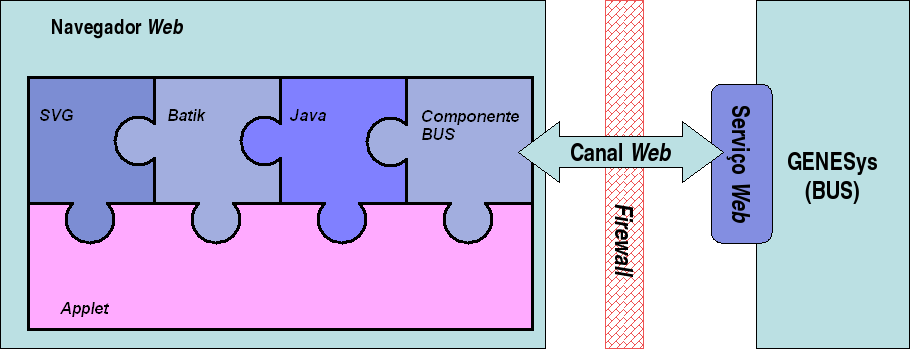
\includegraphics[width=0.86\textwidth]{puzzle}
    \caption{Architecture}
    \label{fig:arch}
\end{figure}

Loren ipsum dolor sit amet, consectetuer adipiscing elit. 
Praesent sit amet sem. Maecenas eleifend facilisis leo. Vestibulum et
mi. Aliquam posuere, ante non tristique consectetuer, dui elit
scelerisque augue, eu vehicula nibh nisi ac est. Nullam laoreet fermentum urna.

Duis eget diam. In est justo, tristique in, lacinia vel, feugiat eget,
quam. Pellentesque habitant morbi tristique senectus et netus et
malesuada fames ac turpis egestas. Fusce feugiat, elit ac placerat
fermentum, augue nisl ultricies eros, id fringilla enim sapien eu
felis. Vestibulum ante ipsum primis in faucibus orci luctus et
ultrices posuere cubilia Curae; Sed dolor mi, porttitor quis,
condimentum sed, luctus in. 

\subsection{Subsection Example} \label{sec:se322}

Suspendisse elementum sodales felis in Table~\ref{tab:example} is a 
floating table.

\begin{table}
  \caption{A table}
\begin{tabular}{|c|r@{.}lr@{.}lr@{.}l||r|}
	\hline
\multicolumn{8}{|c|}
	{\rule[-3mm]{0mm}{8mm}Iteration $k$ de $f(x_n)$} \\
\textbf{\em k}
	& \multicolumn{2}{c}{$x_1^k$}
	& \multicolumn{2}{c}{$x_2^k$}
	& \multicolumn{2}{c||}{$x_3^k$}
	& comments \\ \hline \hline
0   & -0&3                 & 0&6                 &  0&7   & - \\
1   &  0&47102965 & 0&04883157 & -0&53345964  & $\delta<\epsilon$ \\
2   &  0&49988691 & 0&00228830 & -0&52246185  & $\delta < \varepsilon$ \\
3   &  0&49999976 & 0&00005380 & -0&523656   &   $N$ \\
4   &  0&5                 & 0&00000307 & -0&52359743  & \\
\vdots	& \multicolumn{2}{c}{\vdots}
	& \multicolumn{2}{c}{$\ddots$}
	& \multicolumn{2}{c||}{\vdots}  & \\
7   &  0&5   & 0&0    & \textbf{-0}&\textbf{52359878}
		 & $\delta<10^{-8}$ \\ \hline
\end{tabular}
  \label{tab:example}
\end{table}

Loren ipsum dolor sit amet, consectetuer adipiscing elit. 
Praesent sit amet sem. Maecenas eleifend facilisis leo. Vestibulum et
mi. Aliquam posuere, ante non tristique consectetuer, dui elit
scelerisque augue, eu vehicula nibh nisi ac est. Suspendisse elementum
sodales felis. Nullam laoreet fermentum urna. 

Duis eget diam. In est justo, tristique in, lacinia vel, feugiat eget,
quam. Pellentesque habitant morbi tristique senectus et netus et
malesuada fames ac turpis egestas. Fusce feugiat, elit ac placerat
fermentum, augue nisl ultricies eros, id fringilla enim sapien eu
felis. Vestibulum ante ipsum primis in faucibus orci luctus et
ultrices posuere cubilia Curae; Sed dolor mi, porttitor quis,
condimentum sed, luctus in. 

\section{Section Example}

Loren ipsum dolor sit amet, consectetuer adipiscing elit. 
Praesent sit amet sem. Maecenas eleifend facilisis leo. Vestibulum et
mi. Aliquam posuere, ante non tristique consectetuer, dui elit
scelerisque augue, eu vehicula nibh nisi ac est. Suspendisse elementum
sodales felis. Nullam laoreet fermentum urna. 

\section{Summary}

Pellentesque habitant morbi tristique senectus et netus et
malesuada fames ac turpis egestas. Fusce feugiat, elit ac placerat
fermentum, augue nisl ultricies eros, id fringilla enim sapien eu
felis. Vestibulum ante ipsum primis in faucibus orci luctus et
ultrices posuere cubilia Curae; Sed dolor mi, porttitor quis,
condimentum sed, luctus in. 

%%%% Another chapter to force two pages in the index
%%%%
\chapter{Another chapter}

Integer nec quam. Sed fermentum. Nunc vitae leo. Etiam sit amet
quam. Nunc vestibulum massa in mauris. Duis eget nulla. 

\section{Section Example}

Fusce ultricies arcu eu nibh volutpat feugiat. Maecenas urna pede, 
commodo quis, porta eu, bibendum elementum, pede. 

\section{Section Example}

Sed eros massa, molestie eget, mattis non, rutrum ac, magna. 
Duis dui. Maecenas eget tortor ut dolor semper mattis. 
Maecenas auctor, tellus et ultricies tempor, elit
est placerat lacus, in posuere mauris lorem et arcu. 

\subsection{Subsection Example}

Nulla nec eros et pede vehicula aliquam. Aenean sodales pede vel
ante. Fusce sollicitudin sodales lacus. Maecenas justo mauris,
adipiscing vitae, ornare quis, convallis nec, eros. 

\subsection{Subsection Example}

Pellentesque pulvinar fringilla dolor. In sit amet pede. 
Proin orci justo, semper vel, vulputate quis, convallis
ac, nulla. Nulla at justo. Mauris feugiat dolor. 
Etiam posuere fermentum eros. Morbi nisl ipsum, tempus id, 
ornare quis, mattis id, dolor. Aenean molestie metus 
suscipit dolor. Aliquam id lectus sed
nisl lobortis rhoncus. Curabitur vitae diam sed sem aliquet
tempus. Sed scelerisque nisi nec sem.

\section{Section Example}

Sed eros massa, molestie eget, mattis non, rutrum ac, magna. 
Duis dui. Maecenas eget tortor ut dolor semper mattis. 
Maecenas auctor, tellus et ultricies tempor, elit
est placerat lacus, in posuere mauris lorem et arcu. 

\subsection{Subsection Example}

Nulla nec eros et pede vehicula aliquam. Aenean sodales pede vel
ante. Fusce sollicitudin sodales lacus. Maecenas justo mauris,
adipiscing vitae, ornare quis, convallis nec, eros. 

\subsection{Subsection Example}

Aliquam id lectus sed nisl lobortis rhoncus. 
Curabitur vitae diam sed sem aliquet tempus. Sed scelerisque 
nisi nec sem \textcite{khakipoor_linear_2023,liu_energy_2023}.

\section{Section Example}

Maecenas urna pede, commodo quis, porta eu, bibendum elementum, 
pede. Sed eros massa, molestie eget, mattis non, rutrum ac, 
magna. Duis dui. Maecenas eget tortor ut dolor semper mattis. 
Maecenas auctor, tellus et ultricies tempor, elit est placerat 
lacus, in posuere mauris lorem et arcu~\parencite{monopoli_exploiting_2023,zhang_carma_2023,chang_adas_2023, guo_rapidstream_2023}. 

\subsection{Subsection Example}

Nulla nec eros et pede vehicula aliquam. Aenean sodales pede vel
ante. Fusce sollicitudin sodales lacus. Maecenas justo mauris,
adipiscing vitae, ornare quis, convallis nec, eros. 

\subsection{Subsection Example}

Aliquam id lectus sed nisl lobortis rhoncus. 
Curabitur vitae diam sed sem aliquet tempus. Sed scelerisque 
nisi nec sem \textcite{khakipoor_linear_2023,liu_energy_2023} scelerisque.

Nulla nec eros et pede vehicula aliquam. Aenean sodales pede vel
ante. Fusce sollicitudin sodales lacus. Maecenas justo mauris,
adipiscing vitae, ornare quis, convallis nec, eros. Etiam laoreet
venenatis ipsum. In tellus odio, eleifend ac, ultrices vel, lobortis
sed, nibh. Fusce nunc augue, dictum non, pulvinar sed, consectetuer
eu, ipsum. Vivamus nec pede.  

%% Uncomment to see a listing example (cp meic.cfg meec.cfg)
%%%% an example on how to include code
%%% ---------------------------------
\section{Listing example}

Pellentesque habitant morbi tristique senectus et netus et
malesuada fames ac turpis egestas. Fusce feugiat, elit ac placerat
fermentum, augue nisl ultricies eros, id fringilla enim sapien eu
felis.

\begin{lstlisting}[language=Python, caption=Python example, label=code:useless]
# Take the user's input
words = input("Enter the text to translate to pig latin: ")
print(f"You entered: {words}")

# Break apart the words into a list
words = words.split(' ')

# Use a list comprehension to translate words greater than or equal to 3 characters
translated_words = [(w[1:] + w[0] + "ay") for w in words if len(w) >= 3 ]

# Print each translated word
for word in translated_words:
    print(word)
\end{lstlisting}

Listing~\ref{code:useless} uis eget diam. In est justo, tristique in, lacinia vel, feugiat eget,
quam. Pellentesque habitant morbi tristique senectus et netus et
malesuada fames ac turpis egestas. Fusce feugiat, elit ac placerat
fermentum, augue nisl ultricies eros, id fringilla enim sapien eu
felis. Vestibulum ante ipsum primis in faucibus orci luctus et
ultrices posuere cubilia Curae; Sed dolor mi, porttitor quis,
condimentum sed, luctus in.

%%----------------------------------------
%% Final materials
%%----------------------------------------

%% Bibliography
\PrintBib

%% comment next 2 commands if numbered appendices are not used
\appendix
\chapter{Variability of the Segmentation U-Net} \label{ap1:SegmentationUNetVariability}

\begin{table*}[!ht]
	\caption{Dice scores for every vendor and fluid for multiple runs performed in the same conditions. ``Set 1'' resumes Run 1 to Run 5, all of which validated using fold 2. Meanwhile, ``Set 2'' resumes the Runs from 6 to 14, validated in fold 3. All the runs in each set were trained on the same conditions, for 100 epochs. The random transformations applied were horizontal flipping and maximum rotation of $10^{\circ}$ applied to it. This provides an insight of how the randomness of the U-Net affects the segmentation performance.}
	\centering
	\resizebox{\textwidth}{!}{\begin{tabular}{|c|c|ccc|ccc|ccc|c|c|c|c|}
			\hline
			% Headers
			\multirow{2}{*}{\textbf{Runs}} & 
			\multirow{2}{*}{\textbf{VF}} & 
			\multicolumn{3}{c|}{\textbf{Cirrus}} & 
			\multicolumn{3}{c|}{\textbf{Spectralis}} & 
			\multicolumn{3}{c|}{\textbf{Topcon}} & 
			\multicolumn{1}{c|}{\multirow{2}{*}{\textbf{IRF}}} & 
			\multirow{2}{*}{\textbf{SRF}} & 
			\multirow{2}{*}{\textbf{PED}} & 
			\multirow{2}{*}{\textbf{Fluid}} \\ \cline{3-11} & &
			\multicolumn{1}{c}{\textbf{IRF}} & 
			\multicolumn{1}{c}{\textbf{SRF}} & 
			\textbf{\textbf{PED}} & 
			\multicolumn{1}{c}{\textbf{IRF}} & 
			\multicolumn{1}{c}{\textbf{SRF}} & 
			\textbf{PED} & 
			\textbf{IRF} & 
			\textbf{SRF} & 
			\textbf{PED} & 
			\multicolumn{1}{c|}{} & & & \\ 
			
			\hline
			\textbf{Run 1} & 2 & \multicolumn{1}{c|}{0.555} & \multicolumn{1}{c|}{0.773} & 0.634 & \multicolumn{1}{c|}{0.849} & \multicolumn{1}{c|}{0.857} & 0.839 & \multicolumn{1}{c|}{0.783} & \multicolumn{1}{c|}{0.869} & 0.765 & 0.686 & 0.821 & 0.716 & 0.663 \\
			
			\textbf{Run 2} & 2 & \multicolumn{1}{c|}{0.490} & \multicolumn{1}{c|}{0.813} & 0.698 & \multicolumn{1}{c|}{0.786} & \multicolumn{1}{c|}{0.848} & 0.856 & \multicolumn{1}{c|}{0.772} & \multicolumn{1}{c|}{0.903} & 0.834 & 0.639 & 0.850 & 0.773 & 0.692 \\
			
			\textbf{Run 3} & 2 & \multicolumn{1}{c|}{0.349} & \multicolumn{1}{c|}{0.774} & 0.600 & \multicolumn{1}{c|}{0.544} & \multicolumn{1}{c|}{0.799} & 0.759 & \multicolumn{1}{c|}{0.674} & \multicolumn{1}{c|}{0.894} & 0.772 & 0.494 & 0.819 & 0.687 & 0.561 \\
			
			\textbf{Run 4} & 2 & \multicolumn{1}{c|}{0.542} & \multicolumn{1}{c|}{0.776} & 0.677 & \multicolumn{1}{c|}{0.831} & \multicolumn{1}{c|}{0.826} & 0.822 & \multicolumn{1}{c|}{0.852} & \multicolumn{1}{c|}{0.873} & 0.856 & 0.699 & 0.818 & 0.764 & 0.685 \\
			
			\textbf{Run 5} & 2 & \multicolumn{1}{c|}{0.611} & \multicolumn{1}{c|}{0.817} & 0.626 & \multicolumn{1}{c|}{0.832} & \multicolumn{1}{c|}{0.836} & 0.834 & \multicolumn{1}{c|}{0.850} & \multicolumn{1}{c|}{0.913} & 0.822 & 0.732 & 0.853 & 0.730 & 0.685 \\
			
			\hline
			
			\textbf{Set 1} & 2 & \multicolumn{1}{c|}{0.51} & \multicolumn{1}{c|}{0.79} & 0.65 & \multicolumn{1}{c|}{0.77} & \multicolumn{1}{c|}{0.83} & 0.82 & \multicolumn{1}{c|}{0.79} & \multicolumn{1}{c|}{0.89} & 0.81 & 0.65 & 0.83 & 0.73 & 0.66 \\
			
			\hline
			\hline
			
			\textbf{Run 6} & 3 & \multicolumn{1}{c|}{0.661} & \multicolumn{1}{c|}{0.746} & 0.495 & \multicolumn{1}{c|}{0.632} & \multicolumn{1}{c|}{0.842} & 0.736 & \multicolumn{1}{c|}{0.702} & \multicolumn{1}{c|}{0.875} & 0.728 & 0.671 & 0.810 & 0.622 & 0.617 \\
			
			\textbf{Run 7} & 3 & \multicolumn{1}{c|}{0.688} & \multicolumn{1}{c|}{0.622} & 0.596 & \multicolumn{1}{c|}{0.665} & \multicolumn{1}{c|}{0.707} & 0.728 & \multicolumn{1}{c|}{0.846} & \multicolumn{1}{c|}{0.851} & 0.747 & 0.742 & 0.721 & 0.675 & 0.634 \\
			
			\textbf{Run 8} & 3 & \multicolumn{1}{c|}{0.794} & \multicolumn{1}{c|}{0.862} & 0.632 & \multicolumn{1}{c|}{0.663} & \multicolumn{1}{c|}{0.887} & 0.778 & \multicolumn{1}{c|}{0.874} & \multicolumn{1}{c|}{0.833} & 0.780 & 0.801 & 0.856 & 0.712 & 0.719 \\
			
			\textbf{Run 9} & 3 & \multicolumn{1}{c|}{0.622} & \multicolumn{1}{c|}{0.822} & 0.682 & \multicolumn{1}{c|}{0.677} & \multicolumn{1}{c|}{0.846} & 0.758 & \multicolumn{1}{c|}{0.736} & \multicolumn{1}{c|}{0.853} & 0.741 & 0.673 & 0.838 & 0.717 & 0.685 \\
			
			\textbf{Run 10} & 3 & \multicolumn{1}{c|}{0.649} & \multicolumn{1}{c|}{0.718} & 0.671 & \multicolumn{1}{c|}{0.653} & \multicolumn{1}{c|}{0.872} & 0.760 & \multicolumn{1}{c|}{0.828} & \multicolumn{1}{c|}{0.824} & 0.792 & 0.715 & 0.784 & 0.731 & 0.700 \\
			
			\textbf{Run 11} & 3 & \multicolumn{1}{c|}{0.607} & \multicolumn{1}{c|}{0.802} & 0.614 & \multicolumn{1}{c|}{0.669} & \multicolumn{1}{c|}{0.841} & 0.760 & \multicolumn{1}{c|}{0.837} & \multicolumn{1}{c|}{0.864} & 0.787 & 0.702 & 0.831 & 0.703 & 0.697 \\
			
			\textbf{Run 12} & 3 & \multicolumn{1}{c|}{0.565} & \multicolumn{1}{c|}{0.788} & 0.671 & \multicolumn{1}{c|}{0.550} & \multicolumn{1}{c|}{0.868} & 0.755 & \multicolumn{1}{c|}{0.784} & \multicolumn{1}{c|}{0.831} & 0.773 & 0.643 & 0.818 & 0.723 & 0.648 \\
			
			\textbf{Run 13} & 3 & \multicolumn{1}{c|}{0.618} & \multicolumn{1}{c|}{0.699} & 0.406 & \multicolumn{1}{c|}{0.471} & \multicolumn{1}{c|}{0.724} & 0.630 & \multicolumn{1}{c|}{0.752} & \multicolumn{1}{c|}{0.878} & 0.645 & 0.641 & 0.769 & 0.533 & 0.531 \\
			
			\textbf{Run 14} & 3 & \multicolumn{1}{c|}{0.757} & \multicolumn{1}{c|}{0.815} & 0.701 & \multicolumn{1}{c|}{0.646} & \multicolumn{1}{c|}{0.894} & 0.773 & \multicolumn{1}{c|}{0.881} & \multicolumn{1}{c|}{0.848} & 0.836 & 0.783 & 0.841 & 0.763 & 0.738 \\
			
			\hline
			
			\textbf{Set 2} & 3 & \multicolumn{1}{c|}{0.66} & \multicolumn{1}{c|}{0.76} & 0.61 & \multicolumn{1}{c|}{0.63} & \multicolumn{1}{c|}{0.83} & 0.74 & \multicolumn{1}{c|}{0.80} & \multicolumn{1}{c|}{0.85} & 0.76 & 0.71 & 0.81 & 0.69 & 0.66 \\
			
			\hline
			
	\end{tabular}}
	\label{tab:SegmentationUNetVariability}
\end{table*}

\end{document}
